%% sample template file for a MSc Thesis
%% The default is with two sided setup:
\documentclass[%
oneside,    %% uncomment for onesided layout
project,    %% uncomment not thesis but project report
nosummary   %% uncomment if no summary page should be generated
]{USN-MSc}

% The following command removes the chapter names form the header
% (comment/remove) if you prefer to have them:
\pagestyle{plain}

% --- Bibliography setup ---
%%% default is the "ieee" style
\usepackage[style=ieee, sorting=none]{biblatex}
%%% If you want to use "author-year" style
%%% where `\cite{Foo2011}` generates "Foo et al. (2011)"
%%% and   `\parencite{Foo2011}` generates "(Foo et al. 2011)"
%%% then comment the line above and use
%\usepackage[style=authoryear]{biblatex}
%%% or
%%% if you want to use "alphabetic" style then use
%%% where `cite[Foo2011]` generates "[Foo11]"
%%% then comment the line above and use
%\usepackage[style=alphabetic]{biblatex}
%%% instead.
%% load the bib file:
\addbibresource{MscThesis.bib}

\usepackage{lipsum} % just for providing fill text used in this template
\usepackage{array} % for adjusting tables?

% --- general setup ---
%% Please fill in the following parameters:
\newcommand{\mytitle}{%
%% title:
Assignment 2 - Data Visualization and Regression Models
}

\newcommand{\mysubtitle}{%
%% master programme (for thesis only)
%% uncomment the appropriate one:
%Electrical Power Engineering
%Energy and Environmental Technology
Industrial IT and Automation
%Process Technology
}

\newcommand{\mykeywords}{%
%% keywords (for thesis only):
<keyword one, keyword two, \ldots>
}

\newcommand{\myauthor}{%
%% author(thesis) or group code (project):
Lars Rikard Rådstoga
}

\newcommand{\myparticipants}{
%% group participants (for project only)
Lars Rikard Rådstoga
}

\newcommand{\supervisor}{%
%% supervisor:
<Supervisor's Name>}

\begin{document}

% --- title page setup ---
\USNtitlepage%
%% Please provide the following information:
%% #1 optional figure (set to {} if not wanted)
{%
  {\normalsize <optional figure>}
  
\includegraphics[draft,width=\textwidth]{USN_logo_en}}
%% #2 Project partner:
{<Project partner>}
%% #3 Summary:
{%
  \lipsum[6-7]
}

%\chapter*{Preface}
%\label{ch:preface}
%\addcontentsline{toc}{chapter}{Preface}
%\lipsum[1-3]
%\bigskip
%Porsgrunn, \today
%\myauthor %% for thesis
%\myparticipants %% for project


%% table of contents
\tableofcontents
\addcontentsline{toc}{chapter}{\contentsname}

%\listoffigures % out-comment if unwanted
%\addcontentsline{toc}{section}{\listfigurename}

%\listoftables  % out-comment if unwanted
%\addcontentsline{toc}{section}{\listtablename}

%\chapter*{Nomenclature}
%\label{sec:nomenclature}
%bla

%\begin{longtable}{ll}
%  \textbf{Symbol} & \textbf{Explanation}\endhead\\
%  A/D	& Analogue-Digital-Converter \\
%  CMR	& Common Mode Rejection \\
%  foo	& Foo \\
%  bar 	& Bar
%\end{longtable}

\chapter{Understanding the problem}
\label{ch:understanding}
The following chapter discusses and answers a few questions regarding the problem and the dataset, to better understand the following chapters.

\section{What type of problem is it?}
\label{sec:typeOfProblem}
The problem at hand is in fact a regression task. The dataset available contains monitored sensory data, with noise, and can be considered labeled. The goal is to develop a model that can predict/extrapolate the RUL (Remaining Useful Life) of turbofan jet engines.

\section{What category of machine learning is required?}
\label{sec:mlCategory}
As the dataset can be considered labeled, i.e. the columns in the dataset are labeled and have some physical meaning, the supervised learning category will be used.

\section{What does each column in the dataset represent?}
\label{sec:datasetColumns}
The dataset contains multiple columns, see figure \ref{tab:columnDescr} for brief descriptions of each column.

\begin{table}[!ht]
  \caption{Column descriptions}
  \centering
  \begin{tabular}{ | m{3cm} | m{10cm} |}
    \hline
    Engine       & Identification number.                           \\ \hline
    Cycle        & Counted rotations since initialization.          \\ \hline
    Settings 1-3 & How the systems configurations change over time. \\ \hline
    Sensor 1-21  & Various sensor measurements.                     \\ \hline
    RUL          & Remaining useful life.                           \\ \hline
  \end{tabular}
  \label{tab:columnDescr}
\end{table}

\section{Features and targets}
\label{sec:featuresTargets}
Attributes are data types in the dataset that reflect the name of configured or measured values such as voltage set on a motor or pressure. Features are attributes bundled with a value. Targets are usually the information that is intended to predict. In this case features are all configuration, sensory data, and cycle (time). The target is the RUL. The fact that configurations and settings aren't specifically named makes it hard to tell which are important or not.

\section{Not features or targets}
\label{sec:notFeaturesTargets}

Identification columns aren't features if they are all the same brand and make of fan.
Time might be a feature.

\chapter{Data Visualization}
\label{ch:visualization}
This chapter contains visualizations of the dataset that can be used to get better understanding of the system.

\section{Histogram}
\label{sec:histogram}
All the available data was plotted as histograms, see figure \ref{fig:rawHistogram}. Additionally, correlations were investigated using the Pandas Dataframe correlation function.

\begin{figure}[!ht]
  \centering
  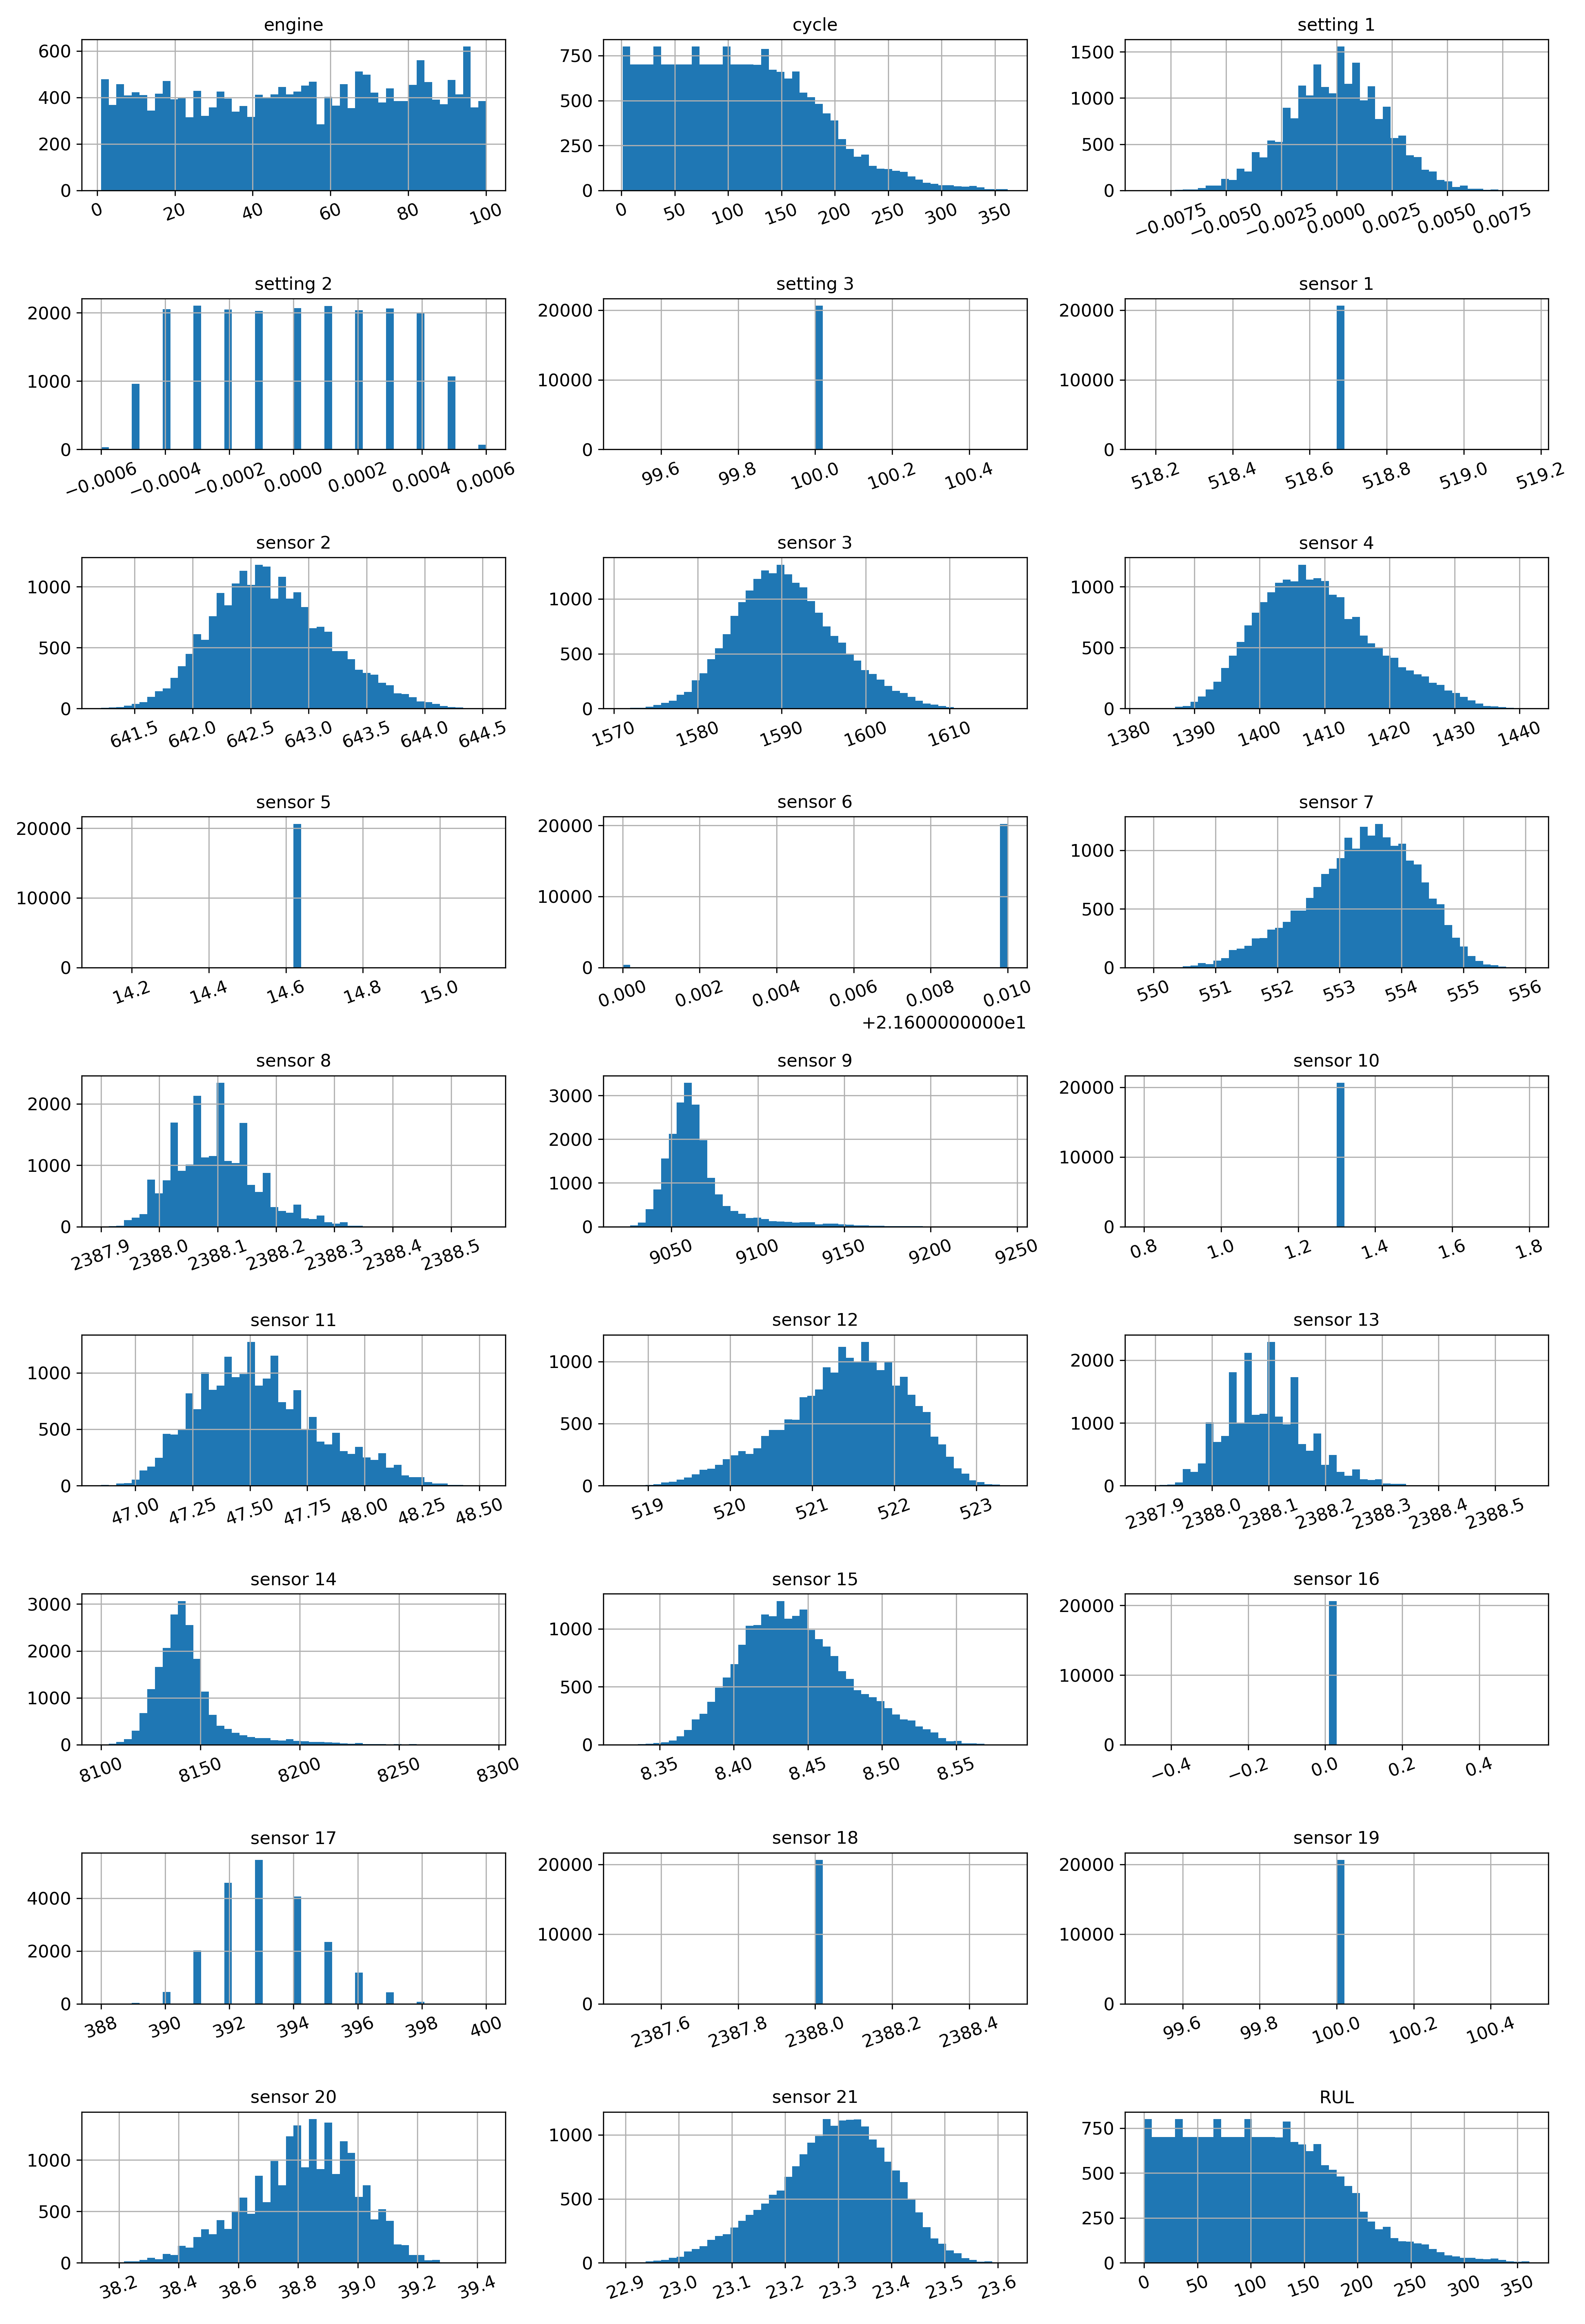
\includegraphics[width=1\textwidth, height=0.9\textheight]{AttributeHistogram}
  \caption{Histogram plot of all attributes.}
  \label{fig:rawHistogram}
\end{figure}

\chapter{Preprocessing and feature selection}
\label{ch:preprocessing}
This chapter discusses the dataset plotted in the previous chapter and which parts of the dataset that should be selected and weather it should be modified.

\section{Feature removal}
\label{sec:featureRemoval}

Initially, some ideas of what features to drop were made through observation of the histogram and the correlation matrix. Following decisions were made:

The engine (ID) attribute is again not a feature or a target, and we can see that most engines have similar amounts of data points, engine attribute could safely be removed.
RUL was removed because it is the target.
Setting 3 and sensors 1, 5, 6, 10, 16, 18, 19 were removed because they all have constant values.
Sensor 7, 11, 12, 15, 17, 20, and 21 were removed because they were too highly correlated to other features, perhaps these are redundant sensors.

Additionally, after running the scikit-learn recursive feature elimination with cross-validation function (RFECV), using a ridge regression estimator, sensor 14 was also deemed unimportant. The reason for using ridge for the estimator here, is to try to avoid bias from using the same regression method as used in later models.

The remaining attributes were then:
Cycle, setting 1 and 2, sensor 2, 3, 4, 8, 9 and 13.

\chapter{Regression models}
\label{ch:regression}
Three different models were created: linear, 2nd degree polynomial, and random forest.

\section{Linear model}
\label{sec:linMod}

\section{2nd degree polynomial model}
\label{sec:polMod}

\section{Random forest model}
\label{sec:rfMod}

\chapter{Regression models with extended features}
\label{ch:regressionExtended}
\lipsum[1]


% A dummy command that causes all bibliographyentries to be displayed
% even though there were not cited in the document. Used for demonstration
% purposes only in this template file.
~\nocite{*}

\cleardoublepage

% The bibliography should be displayed here...
%\printbibliography[heading=bibintoc]
% You rather like to call the bibliography "References"? Then use this instead:
\printbibliography[heading=bibintoc, title={References}]


\appendix
%%\renewcommand{\appendixname}{Paper} %% So we get 'Paper X' displayed instead
%
%
%\chapter[Short Title of Paper A]{Title of Paper A (probably very long and therefore not good to have in the header)}
%\label{paper-a}
%
%\paragraph{Note}
%Since some papers tend to have a rather long title it is good to provide the optional short title which then will be displayed in the table of contents and header instead of the long original title.
%On the openening page of the chapter the orginal \emph{long} title will be displayed.\bigskip
%
%\emph{Short descriptive text of paper follows here.}\bigskip
%
%The paper itself needs to be included in the published form as PDF on the next pages.
%This can be done using the \texttt{pdfpages} package by adding the command:
%
%\begin{verbatim}
%\includepdf{pages=-,openright}{Filename}
%\end{verbatim}
%
%You can omit the \texttt{.pdf} when specifying the \texttt{Filename}. Also you should include always include the option \texttt{openright} since it would look strange to have the paper starting at the back of the cover page.
%
%There are more options like only adding specific pages:
%\begin{verbatim}
%\includepdf{pages=2-6,openright}{Filename.pdf}
%\end{verbatim}
%
%For more options see Appendix~\ref{paper-b} where the most important pages of the \texttt{pdfpages} manual were inlcuded using \texttt{pdfpages}.
%
%
%%%% Command to include a PDF file directly including all pages:
%
%
\chapter[Source code]{Source code}
\label{app:sourceCode}
%Short descriptive text of paper follows here.
The source code, Jupyter notebook, used to load, transform and plot data.
%Here we included the first five pages of the \texttt{pdfpages} manual itself.
%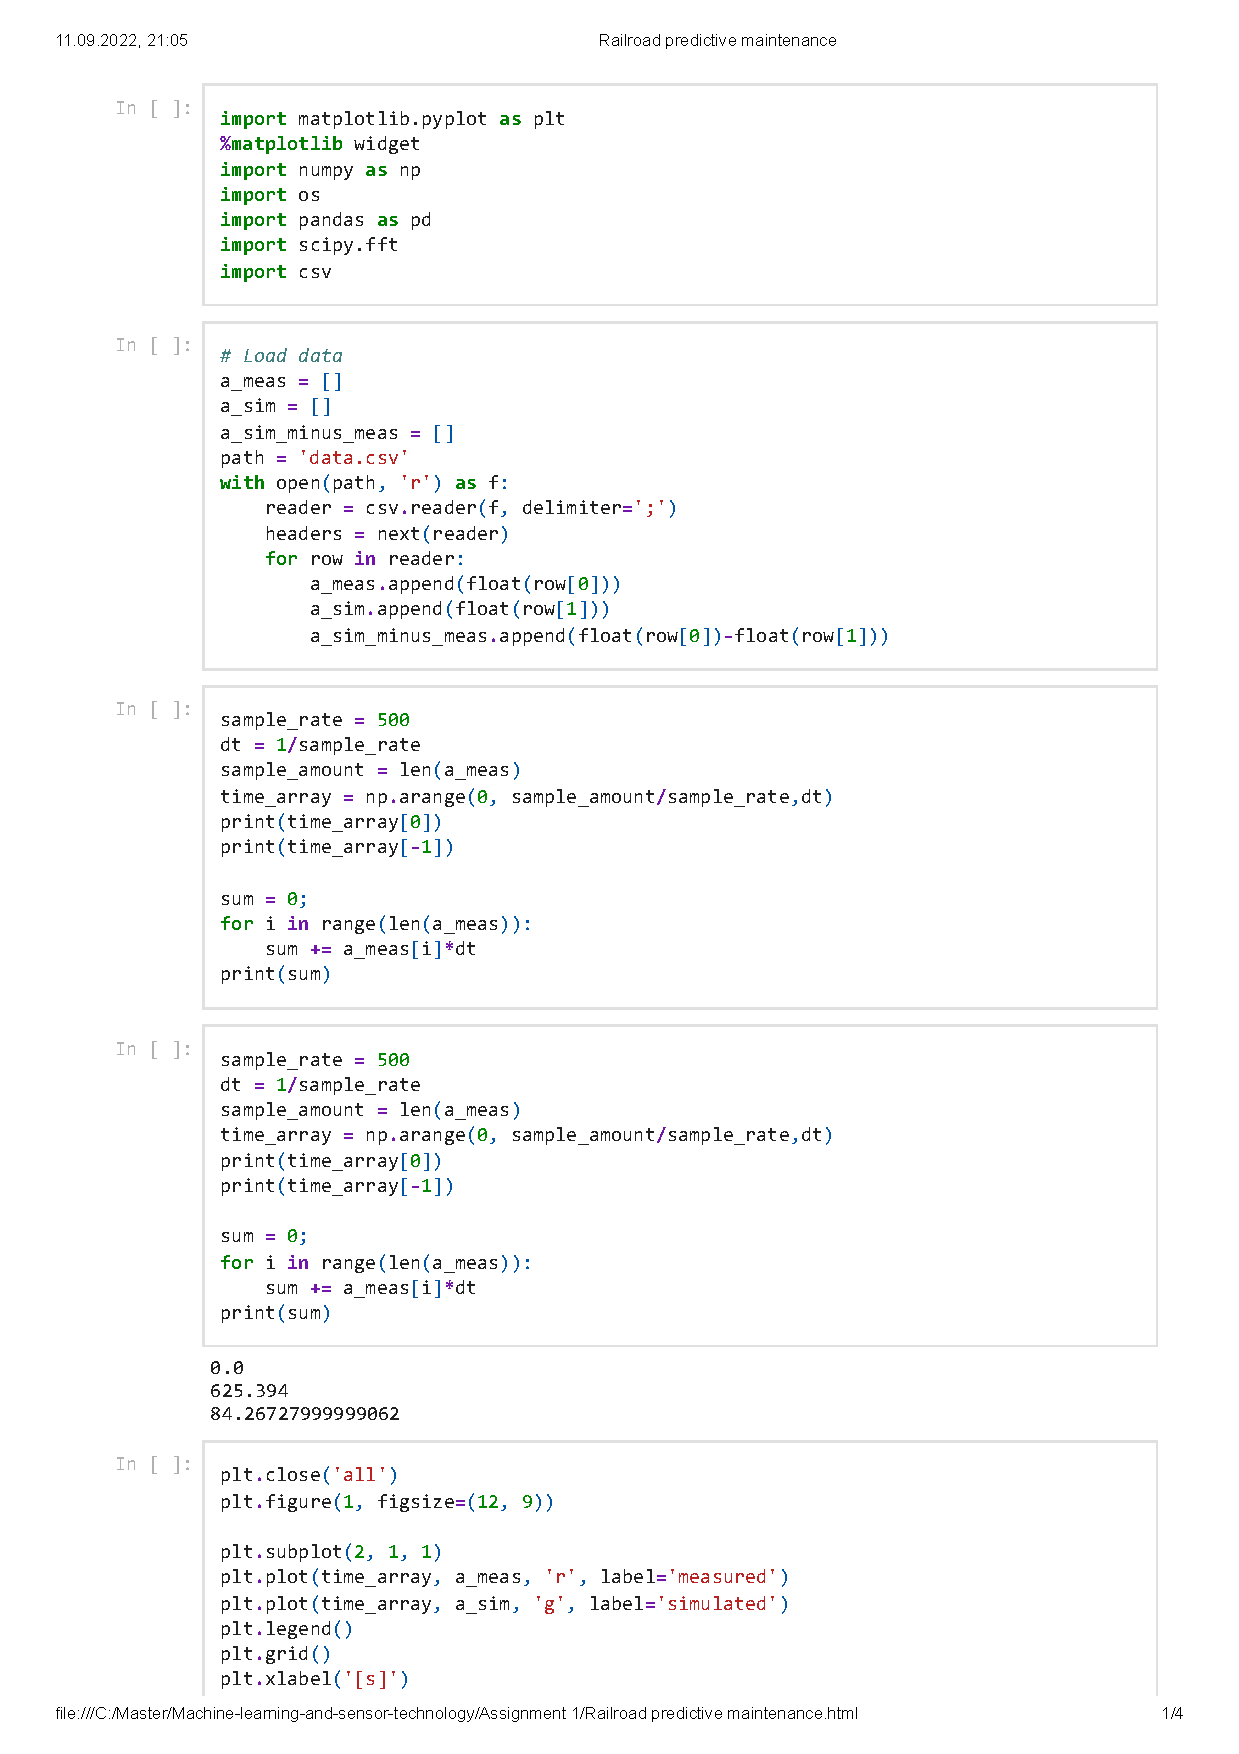
\includepdf[pages=1-4,openright]{fig/Railroad predictive maintenance}
\end{document}

%%% Local Variables:
%%% mode: latex
%%% TeX-master: t
%%% End:
